\chapter{Evaluation of results}


The hyperparameter optimization and model selection process was run on a number of datasets that
include 29 standard datasets commonly used in the machine learning community, and 8 datasets taken from
biological experiments. The datasets were also analyzed under the default settings for all SML
algorithms.

The SML algorithms applied on the datasets were: PassiveAggressive, RadiusNeighbors, GaussianNB,
ExtraTreeEnsemble, SVM, LinearDiscriminant, KNN, RandomForest,
StochasicGradientDescent, LogisticRegression, NearestCentroid, 
LinearSVM, NuSVM, DecisionTree,
Ridge, QuadraticDiscriminant, and 
GradientBoosting.


The optimization stage for each of the datasets was run during 8 hours as distributed tasks on the
Brutus Cluster.

A comparison between the performance indices obtained by using default and optimized hyperparameters
is show in table \ref{tb:comparison_all}.

In general, the performance indices of the optimized models are significantly higher than the
performance indices under the default configurations. A few datasets did not show improvement over
the default settings. In these cases, the best classification performance was obtained by using the
LinearDiscriminant classifier, which does not expose any hyperparameters to configure.

The table shows that the SML algorithm that performs best and improvement over the default settings stictly
depends on the dataset.

%\begin{figure}
%	\begin{centering}
%		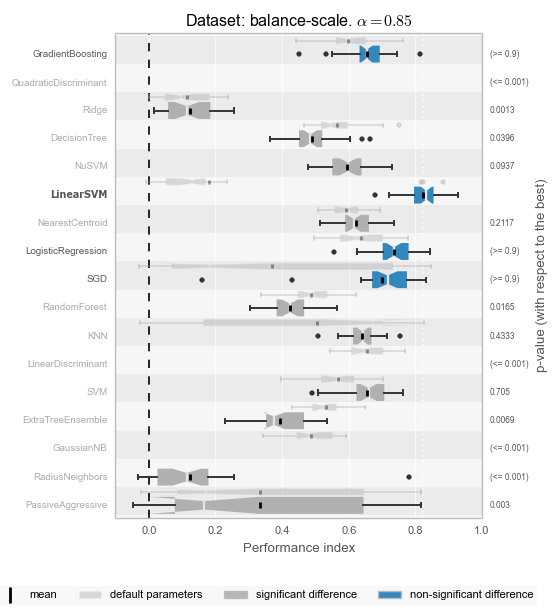
\includegraphics[width=\textwidth]{optimized_vs_default}
%	\end{centering}
%	\caption{blablabla}
%\end{figure}
%

\begin{table}[h!]
\centering
\begin{tabularx}{\textwidth}{l r r r r r l}
	& \multicolumn{2}{c}{\bf default} & ~ & \multicolumn{3}{c}{\bf Optimized}\\
	\cline{2-3}
	\cline{5-7}
{\bf Dataset} & Worst & Best & ~ & Score & Boost & Family\\
	\cline{1-7}
	\input{images/comparison_table.txt}
\end{tabularx}
\caption{Comparison of optimized and default performance indices for all datasets.}
\label{tb:comparison_all}
\end{table}

\section{Results on standard Machine Learning datasets}

Standard datasets are commonly used for testing and evaluating machine learning approaches. Some of
the datasets used here are inherently difficult to classify, and hence most SML algorithms
consistently obtain a very low performance index; other datasets are simple to classify and hence
good performance indices but little improvement over the default values is expected.

Figure \ref{img:optvsdefstandard} shows an example of the distribution of performance indices for
different models, and their shift with respect to the performance indices obtained by the default
models, for a specific dataset. Each row in the plot corresponds to a different algorithm under the
default (thin boxplots) and optimized settings. Distributions that are not significantly different
from the best, up to a level $\alpha$ shown on the title of the plot, are highlighted. The p-values
reported by the statistical test are displayed on the right side of the plot. Models with p-values
above the $\alpha$ level are considered statistically indistinguishable.

The baseline is shown as a vertical dotted line. It is possible for some models to score lower than the
baseline, as explained in section \ref{sec:performance_measurement}.

In cases where algorithms do not work at all on a given dataset, their performance indices are
reported as a single point over the baseline.

\begin{figure}[h!]
	\centering
	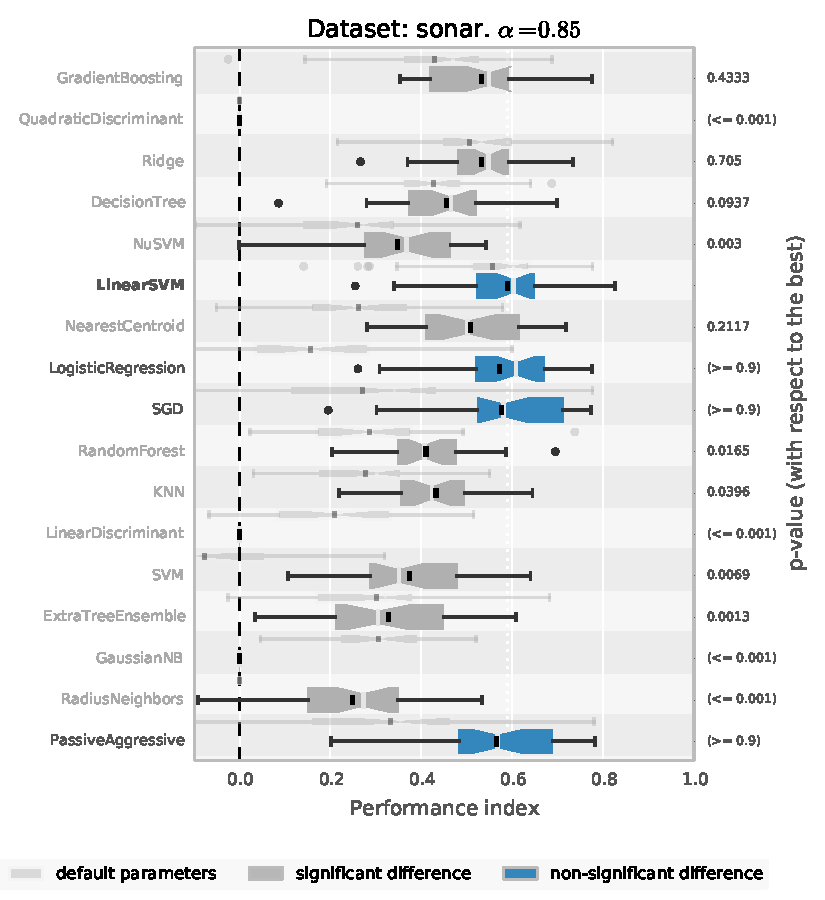
\includegraphics{optimized_vs_default_standard}
	\caption{Optimized vs default values for a standard machine learning dataset}
	\label{img:optvsdefstandard}
\end{figure}


\section{Results on biological data}

\begin{figure}[h!]
	\centering
	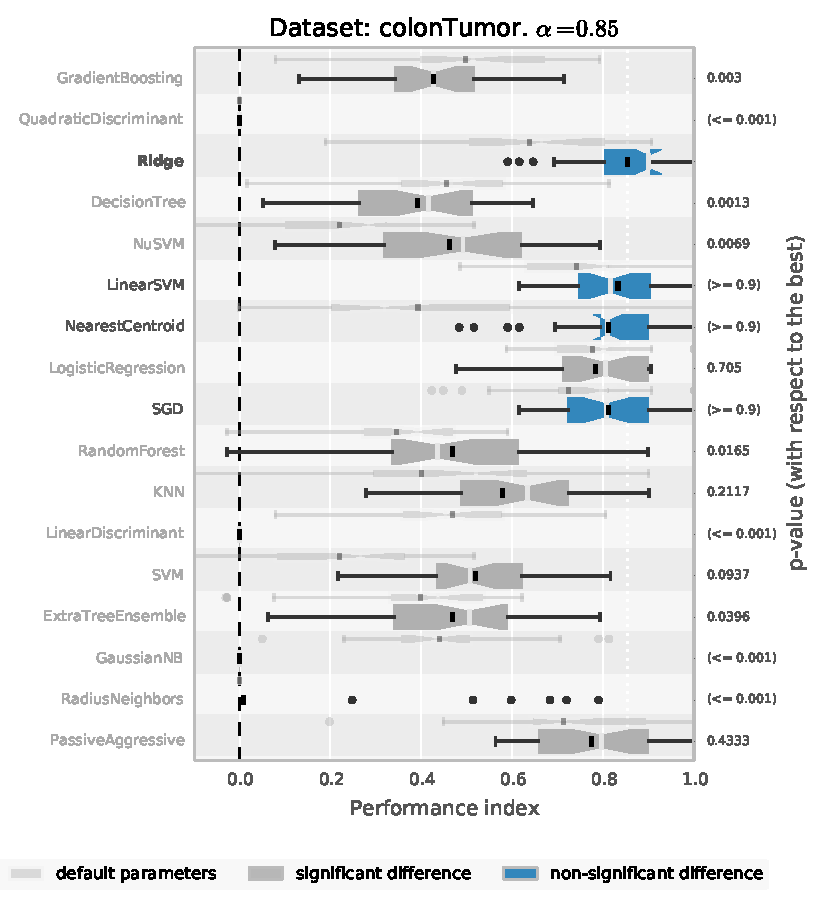
\includegraphics{optimized_vs_default_bio}
	\caption{Optimized vs default values for a biological dataset}
	\label{img:optvsdefbio}
\end{figure}

\section{General prior learning}

The 29 standard machine learning datasets were used to learn general priors for all numerical
hyperparameters on all SML algorithms, as explained in \ref{sec:learning_prior}. 

Gammas from poly approx uniform, gammas from sigmoid: skewed


\begin{figure}[h!]
	\centering
	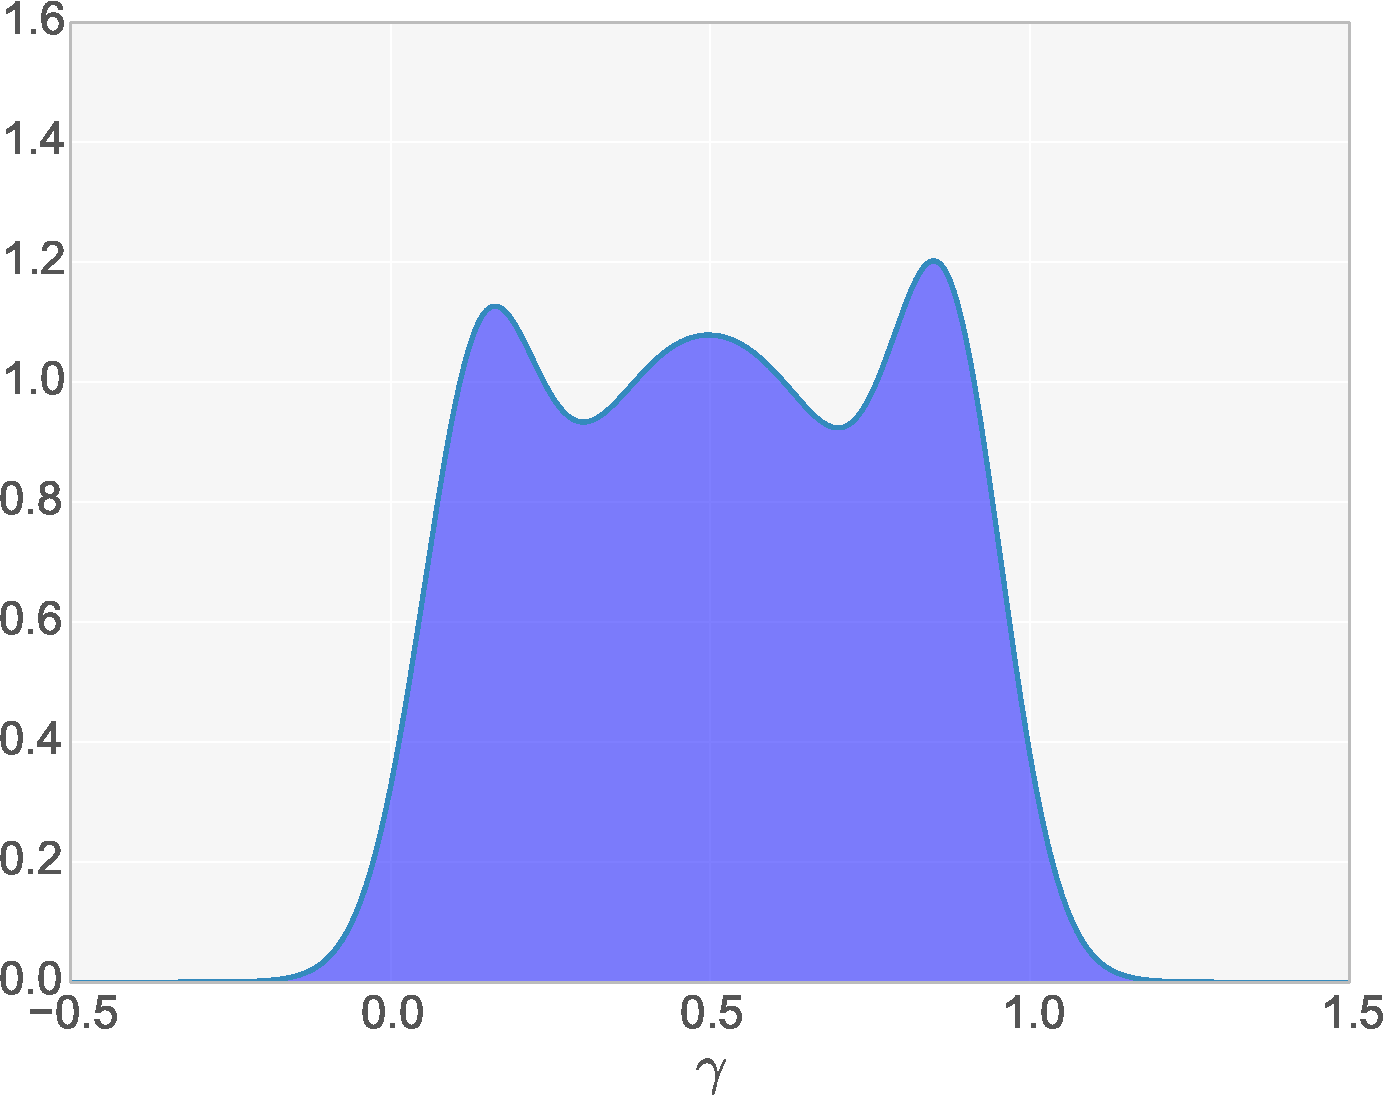
\includegraphics[width=.3\textwidth]{learned1}
	\caption{gamma for signature auto\_sigmoid\_True}
	\label{img:learned1}
\end{figure}


\begin{figure}[h!]
	\centering
	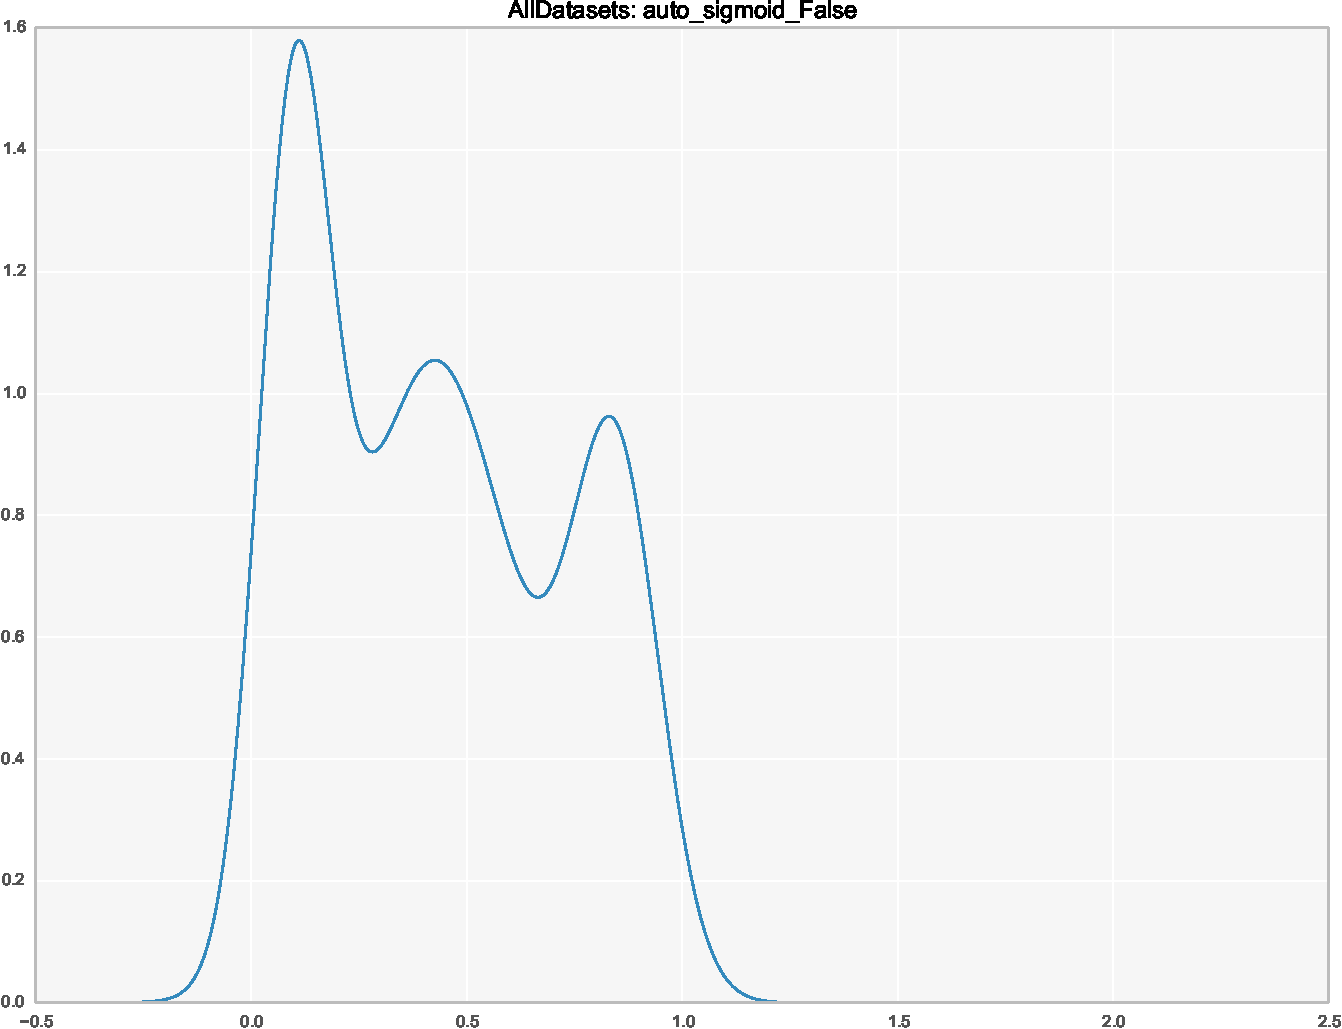
\includegraphics[width=.3\textwidth]{learned2}
	\caption{learner distribution 2}
	\caption{gamma for signature auto\_sigmoid\_False}
	\label{img:learned2}
\end{figure}


\begin{figure}[h!]
	\centering
	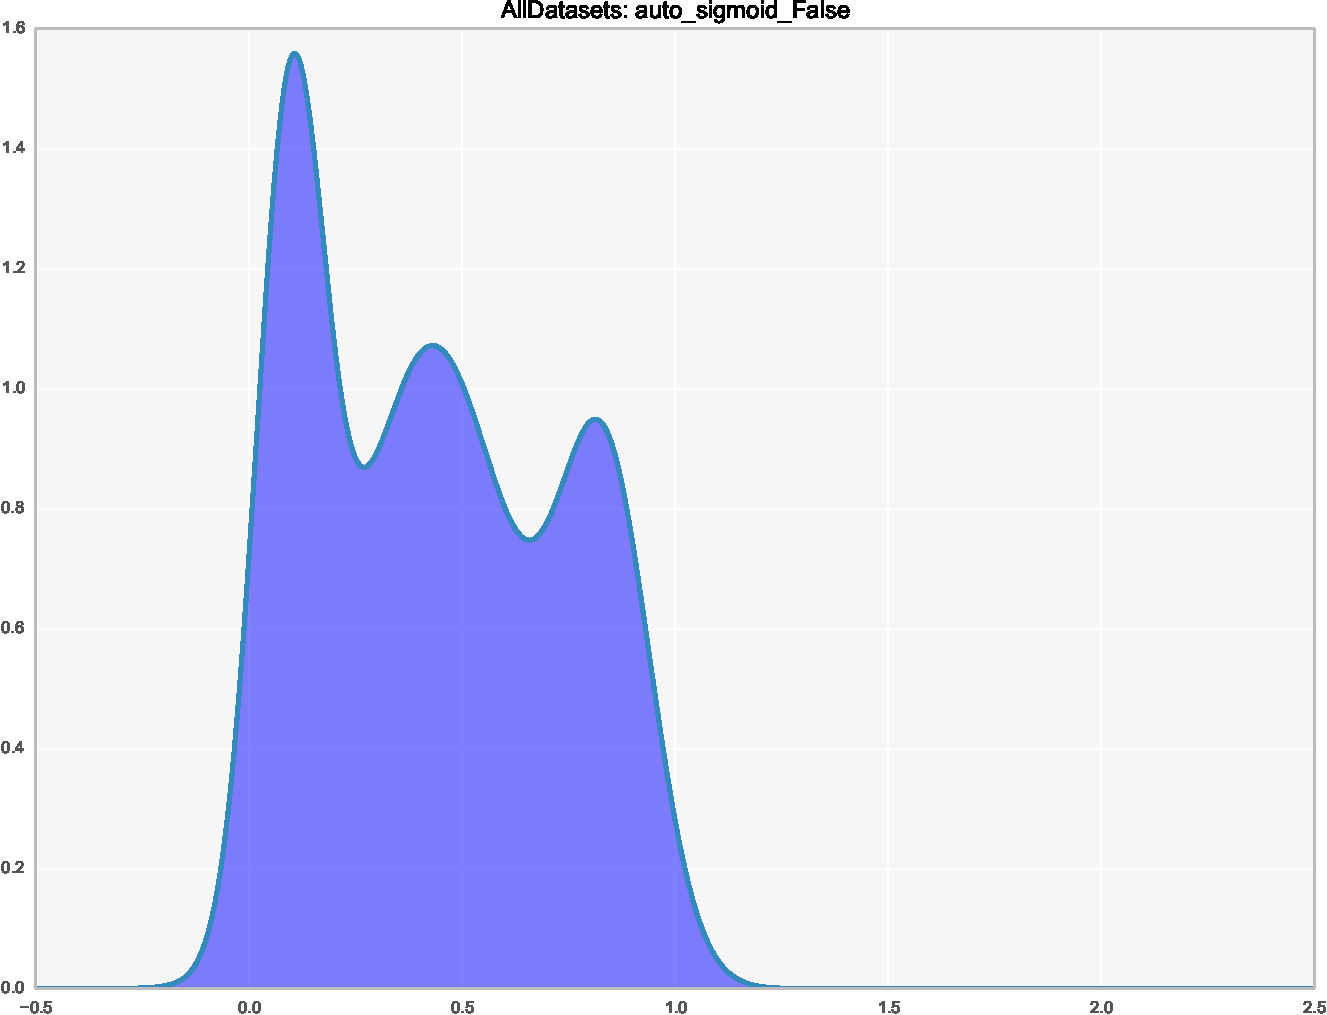
\includegraphics[width=0.3\textwidth]{learned3}
	\caption{gamma for signature auto\_poly\_True}
	\label{img:learned3}
\end{figure}


\begin{figure}[h!]
	\centering
	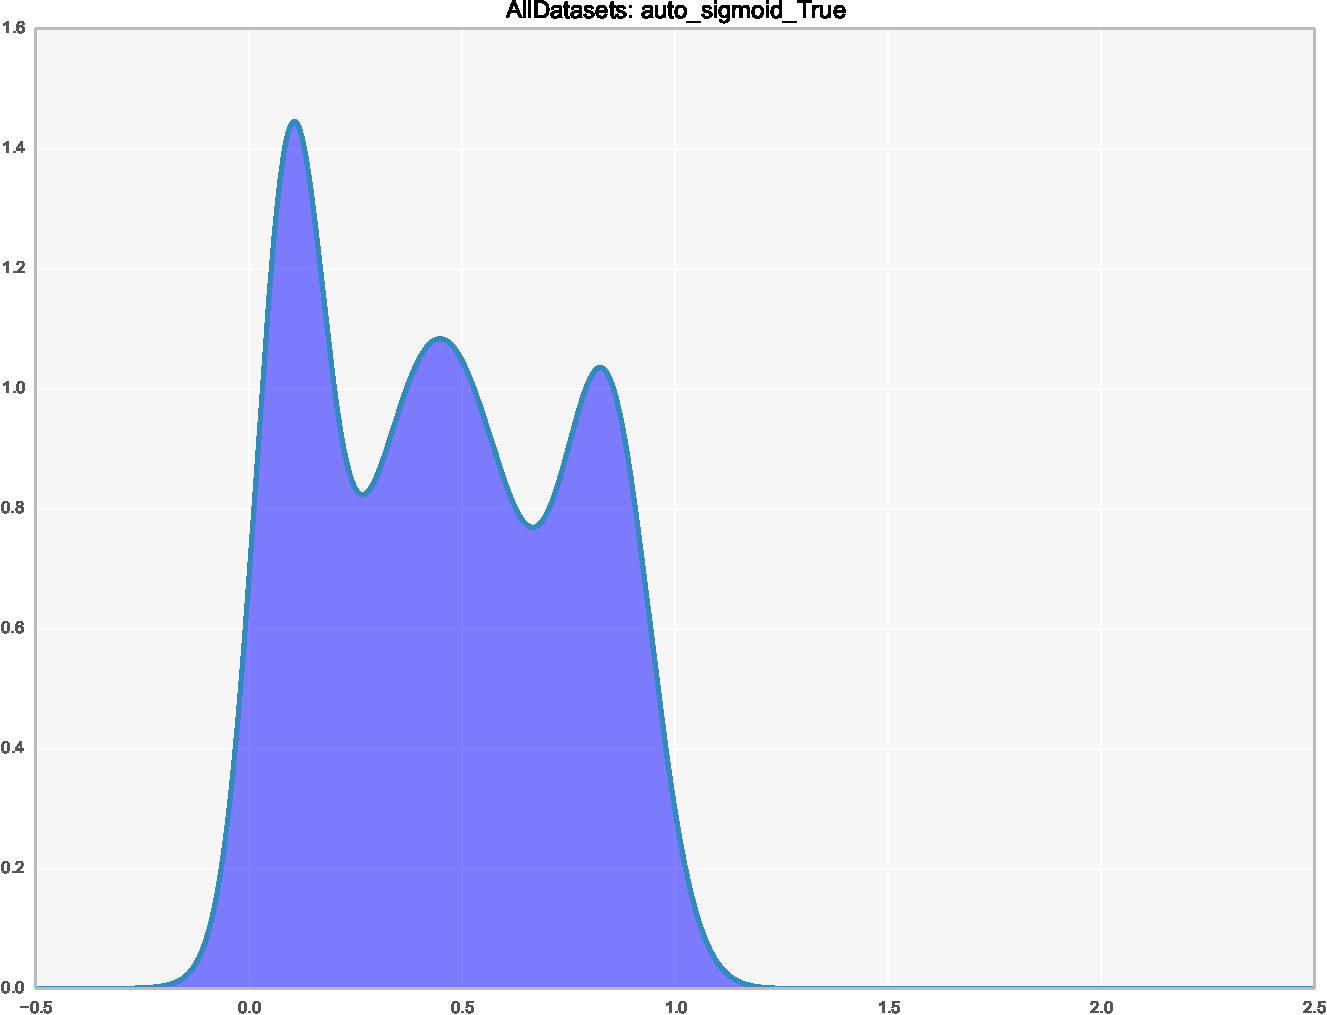
\includegraphics[width=.3\textwidth]{learned4}
	\caption{gamma for signature auto\_poly\_False}
	\label{img:learned4}
\end{figure}


